\section{Accessibility}
The Executive Council of SIGCHI has committed to making SIGCHI
conferences more inclusive for researchers, practitioners, and
educators with disabilities. As a part of this goal, the all authors
are asked to work on improving the accessibility of their
submissions. Specifically, we encourage authors to carry out the
following five steps:
\begin{itemize}\compresslist%
\item Add alternative text to all figures
\item Mark table headings
\item Generate a tagged PDF
\item Verify the default language
\item Set the tab order to ``Use Document Structure''
\end{itemize}

For links to instructions and resources, please see:
\url{http://chi2016.acm.org/accessibility}

Unfortunately good tools do not yet exist to create tagged PDF files
from Latex. \LaTeX\ users will need to carry out all of the above
steps in the PDF directly using Adobe Acrobat, after the PDF has been
generated.

For more information and links to instructions and resources, please
see:
\url{http://chi2016.acm.org/accessibility}.

% \begin{figure*}
%   \centering
%   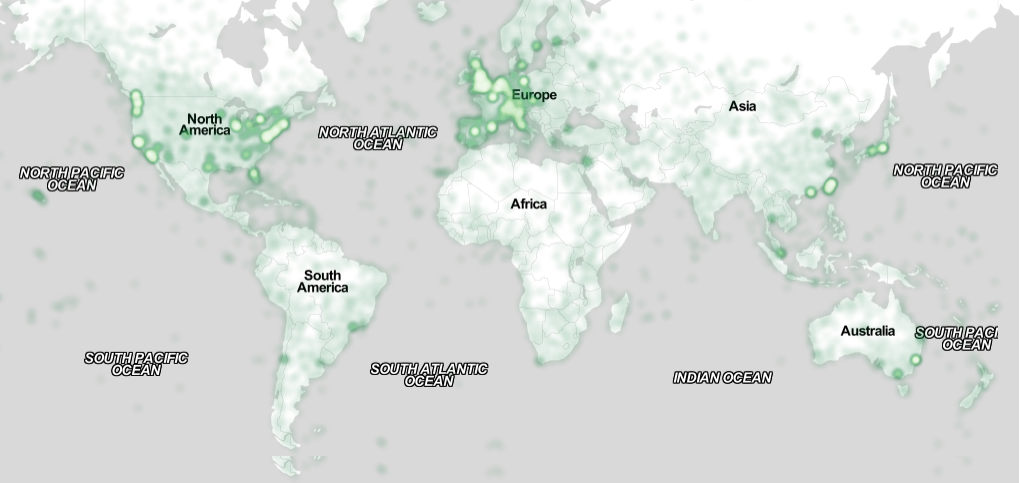
\includegraphics[width=1.3\columnwidth]{figures/map}
%   \caption{In this image, the map maximizes use of space. You can make
%     figures as wide as you need, up to a maximum of the full width of
%     both columns. Note that \LaTeX\ tends to render large figures on a
%     dedicated page. Image: \ccbynd~ayman on Flickr.}~\label{fig:cats}
% \end{figure*}
